\documentclass{beamer}

% Draft (faster compilation, no images)
%\documentclass[draft]{beamer}

% Notes on the right
%\usepackage{pgfpages}
%\setbeameroption{show notes on second screen=right}

% Handout, no overlays
%\documentclass[handout]{beamer}

%\usepackage[utf8]{inputenc}
\usepackage[english]{babel}

\usetheme[
%  sectionpage=none,
  subsectionpage=none,
  numbering=fraction,
  progressbar=foot
]{metropolis}
\usecolortheme{owl} % Dark theme
\setmonofont{Inconsolata}
\definecolor{PowerDNSOrange}{RGB}{233,102,25}

% Some Open-Xchange colors
\definecolor{OXOrange}{RGB}{230,110,0}
\definecolor{OXGraphiteBlack}{RGB}{45,45,45}
\definecolor{OXSilverGrey}{RGB}{220,220,220}
\definecolor{OXGrey}{RGB}{135,135,135}

\definecolor{ProgressBarBG}{RGB}{238,238,236}
\setbeamercolor{progress bar}{fg=PowerDNSOrange, bg=OXGrey}

% Webicons
\usepackage{fontawesome}

\usepackage{shellesc}
\usepackage{minted}
\usemintedstyle{native}
\setminted[lua]{
  linenos=true,
  breaklines=true,
  frame=lines,
  fontsize=\footnotesize
}
\setminted[shell]{ % used for output
  style=bw,
  fontsize=\tiny
}
\renewcommand{\theFancyVerbLine}{\ttfamily
  \textcolor[rgb]{0.5,0.5,1.0}{\scriptsize
  \arabic{FancyVerbLine}}}

% Non-retarded image import
\usepackage{graphicx}

% PDF niceness
\usepackage{hyperref}

% No nav symbols on the PDF
\beamertemplatenavigationsymbolsempty

\title[aname]{xpf: DNS X-Proxied-For (draft-bellis-dnsop-xpf-02)}
\author{\textbf{Peter van Dijk}\\Senior PowerDNS Engineer\\with Ray Bellis and Rémi Gacogne}
\date{}
\titlegraphic{
\vfill\large{\href{https://twitter.com/Habbie}{\faicon{twitter-square}~Habbie} \hfill \href{https://github.com/Habbie}{Habbie~\faicon{github-square}}}\\
              \small{\href{https://twitter.com/PowerDNS}{\faicon{twitter-square}~PowerDNS} \hfill \href{https://github.com/PowerDNS}{PowerDNS~\faicon{github-square}}}\\
              \vspace{150px}
              \center{
\includegraphics[width=.4\textwidth]{img/powerdns-logo.eps}}
}

\hypersetup{
  pdfauthor={Peter van Dijk},
  pdfsubject={},
  pdftitle={DNS X-Proxied-For},
  pdfkeywords={xpf dns dnsop}
}

\begin{document}

\begin{frame}
  \titlepage
\end{frame}

\begin{frame}{Traditional setup}
  \center{
    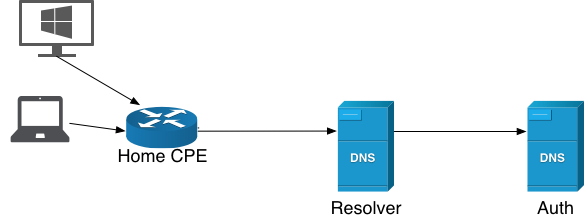
\includegraphics[width=.95\textwidth]{img/Canvas1.png}
  }
\end{frame}

\begin{frame}{plus ECS}
  \center{
    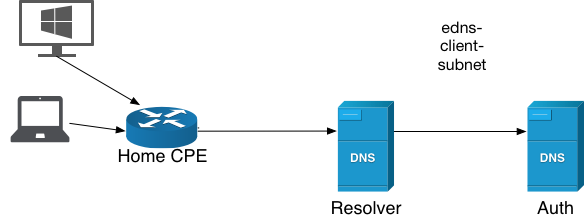
\includegraphics[width=.95\textwidth]{img/Canvas2.png}
  }
\end{frame}

\begin{frame}{add a firewall/balancer/TLS unwrapper}
  \center{
    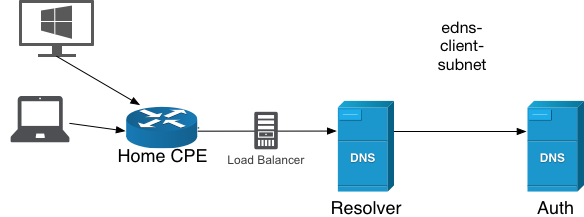
\includegraphics[width=.95\textwidth]{img/Canvas3.png}
  }
\end{frame}

\begin{frame}{reinstate seeing client IP}
  \center{
    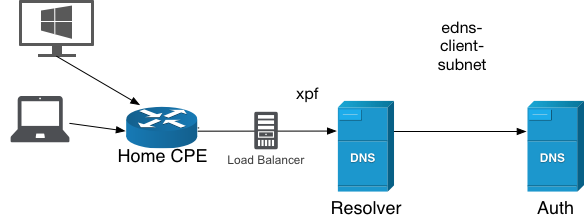
\includegraphics[width=.95\textwidth]{img/Canvas4.png}
  }
\end{frame}

\begin{frame}{auth operator also needs a firewall/balancer}
  \center{
    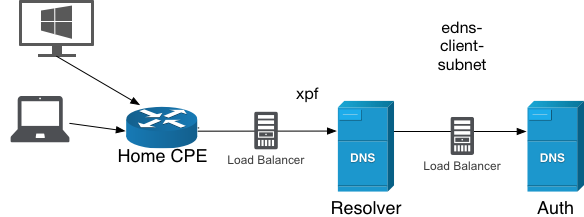
\includegraphics[width=.95\textwidth]{img/Canvas5.png}
  }
\end{frame}

\begin{frame}{thus also needs xpf}
  \center{
    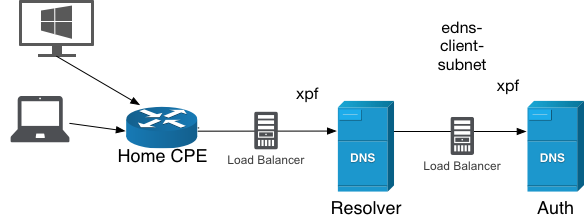
\includegraphics[width=.95\textwidth]{img/Canvas6.png}
  }
\end{frame}

\begin{frame}{boundaries}
  \center{
    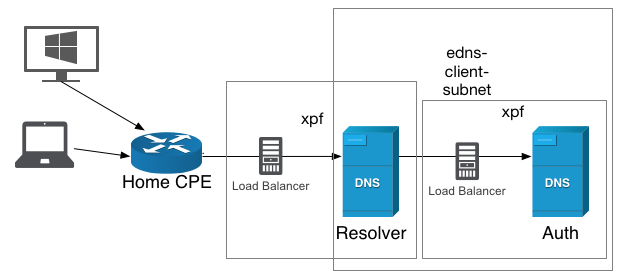
\includegraphics[width=.95\textwidth]{img/Canvas7.png}
  }
\end{frame}

\begin{frame}{for reference, clientid}
  \center{
    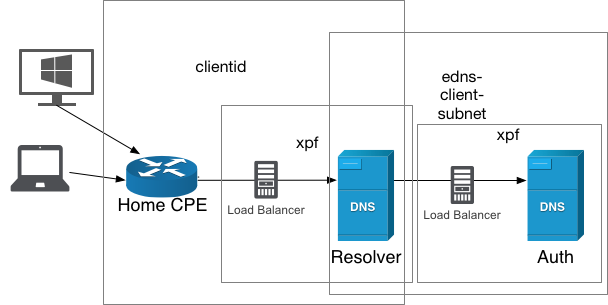
\includegraphics[width=.95\textwidth]{img/Canvas8.png}
  }
\end{frame}

\begin{frame}{Record format}
  \center{
    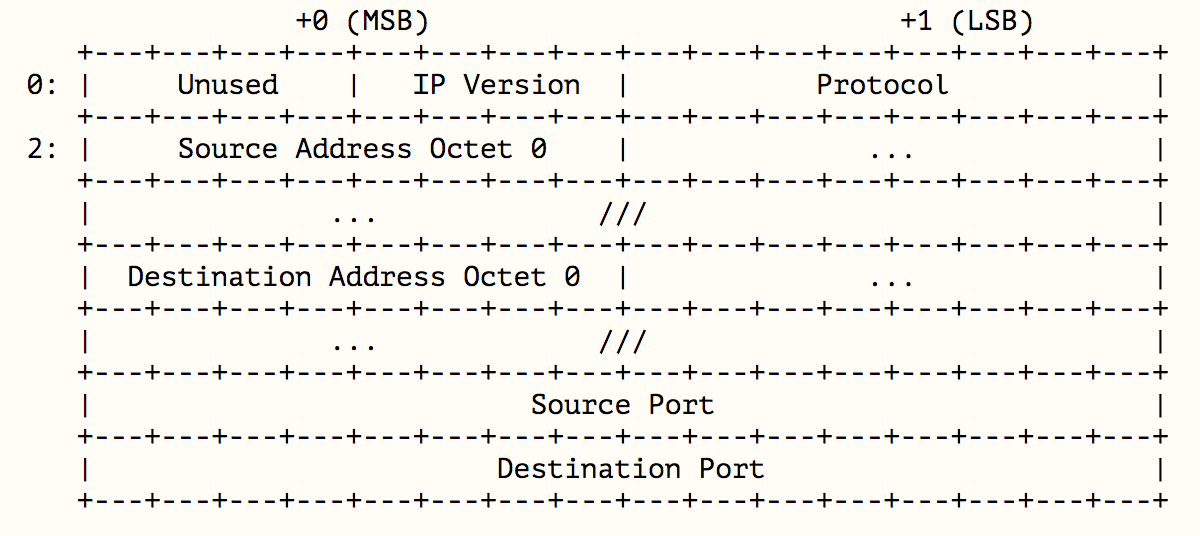
\includegraphics[width=.95\textwidth]{img/record.png}
  }
\end{frame}

\begin{frame}{Concerns}
  \begin{itemize}
    \item ...
  \end{itemize}
\end{frame}

\begin{frame}{Next steps}
  \begin{itemize}
    \item get some code running
    \item ...
  \end{itemize}
\end{frame}

\begin{frame}{Questions?}
Questions? Comments?

\end{frame}

\end{document}
